\documentclass[10pt]{article}
% Course cheatsheet: estimands, assumptions, and results of Meetings 1 to 11 on six landscape pages.
% Every Result is stated as in the technical notes; notation follows shared/notation.tex.
\usepackage[letterpaper,landscape,top=0.56in,bottom=0.5in,left=0.4in,right=0.4in,headsep=0.12in,footskip=0.28in]{geometry}
\usepackage{amsmath,amssymb,mathtools,bm}
\usepackage[T1]{fontenc}
\usepackage[sc]{mathpazo}
\usepackage{microtype}
\usepackage{multicol}
\usepackage{booktabs,tabularx,array}
\usepackage{xcolor}
\usepackage{enumitem}
\usepackage{pifont}
\usepackage{adjustbox}
\usepackage{fancyhdr}
\usepackage{tikz}
\usetikzlibrary{arrows.meta,positioning,calc}
\usepackage[colorlinks=true,linkcolor=noteblue,urlcolor=noteblue]{hyperref}

\definecolor{sbgreen}{HTML}{00704A}
\definecolor{noteblue}{HTML}{2060A0}
\definecolor{warnred}{HTML}{B42318}
\definecolor{greentint}{HTML}{EEF6F2}
\definecolor{extgrey}{HTML}{6B7280}

\newcommand{\E}{\mathbb{E}}
\newcommand{\Var}{\operatorname{Var}}
\newcommand{\Cov}{\operatorname{Cov}}
\newcommand{\indep}{\perp\!\!\!\perp}
\newcommand{\ind}[1]{\mathbf{1}\{#1\}}
\newcommand{\hatt}{\hat{\tau}}
\newcommand{\SE}{\operatorname{SE}}
\newcommand{\ATE}{\text{ATE}}
\newcommand{\ATT}{\text{ATT}}
\newcommand{\ATU}{\text{ATU}}

% ---- Layout ------------------------------------------------------------------------------------
\linespread{0.95}
\setlength{\columnsep}{0.32in}
\setlength{\parindent}{0pt}
\setlength{\parskip}{0.22em}
\setlist{itemsep=0.05em,topsep=0.15em,leftmargin=1.1em}
\newcolumntype{L}[1]{>{\raggedright\arraybackslash}p{#1}}
\renewcommand{\arraystretch}{1.04}

\pagestyle{fancy}
\fancyhf{}
\fancyhead[L]{\small\textsc{SHBI-GB 7342 \quad Applied Causal Inference for Business}}
\fancyhead[R]{\small\textsc{Cheatsheet}}
\fancyfoot[L]{\small\textsc{Zhikun Lu}}
\fancyfoot[C]{\small\thepage}
\fancyfoot[R]{\small\textsc{Fall 2026}}
\renewcommand{\headrulewidth}{0.4pt}

\makeatletter
\renewcommand{\section}{\@startsection{section}{1}{0pt}{0.75em plus 0.2em}{0.3em}{\large\bfseries\color{sbgreen}}}
\renewcommand{\subsection}{\@startsection{subsection}{2}{0pt}{0.45em plus 0.1em}{0.15em}{\normalsize\bfseries}}
\makeatother

% An entry: a box glyph, the term in bold, then the definition or result.
\newcommand{\term}[1]{\par\vspace{0.12em}{\color{sbgreen}\ding{113}}\,\textbf{#1.}\ }
% A remark in the example's blue italic.
\newcommand{\remark}[1]{\par{\color{noteblue}\itshape\small Remark: #1}\par}
% A boxed key formula, centered.
% max width keeps a box inside the column even if a formula is too long
\newcommand{\keybox}[1]{\par\smallskip{\centering\adjustbox{max width=\linewidth}{\fcolorbox{sbgreen}{greentint}{\ensuremath{\displaystyle #1}}}\par}\smallskip}

\tikzset{n/.style={circle,draw,inner sep=1.2pt,minimum size=0.5cm,font=\small},
         a/.style={-{Stealth[length=4pt]},thick}}

\begin{document}
\begin{multicols*}{2}
\raggedcolumns

% ================================================================================================
\begin{center}
{\LARGE Cheatsheet:\\[0.15em] Applied Causal Inference for Business}\\[0.5em]
{\large Zhikun Lu}\\[0.2em]
{\normalsize SHBI-GB 7342 \quad Fall 2026}
\end{center}

{\itshape This cheatsheet collects the estimands, assumptions, and main results of Meetings 1 to 11 in the course notation.
Results are stated as in the course; their proofs, worked examples, and exercises are not repeated here. The course asks one
question throughout: where does the counterfactual, what would have happened without the action, come from?}

\begin{center}
\small
\begin{tabular}{@{}lL{4.1cm}L{3.6cm}@{}}
\toprule
\textbf{Meetings} & \textbf{The comparison comes from} & \textbf{What may be unobserved} \\
\midrule
1--5 & a randomized control group & anything \\
6--8 & units that look alike on measured variables & nothing relevant \\
9 & a simulator learned from logs, with the effect planted & nothing relevant (the 6--8 assumption, made explicit) \\
10--11 & untreated units observed over time & time-stable confounders \\
\bottomrule
\end{tabular}
\end{center}

% ================================================================================================
\section{Causal basics (Meeting 1)}

\subsection{Potential outcomes and estimands}

\term{Potential outcomes} Each unit $i$ has an outcome $Y_i(1)$ if treated and $Y_i(0)$ if not. Its effect is
$\tau_i = Y_i(1) - Y_i(0)$. Only one potential outcome is ever observed: $Y_i = D_iY_i(1) + (1-D_i)Y_i(0)$ (consistency).

\term{Estimand} A summary of potential outcomes for a named population. It specifies the units, the intervention and its
comparator, the outcome and its horizon. It is fixed before, and independently of, any data or method.

\term{Average effects} $\ATE = \E[\tau_i]$, $\ATT = \E[\tau_i \mid D_i = 1]$, $\ATU = \E[\tau_i \mid D_i = 0]$. With
$\pi = \Pr(D=1)$, $\ATE = \pi\,\ATT + (1-\pi)\,\ATU$.

\term{Response types} For a binary outcome, every unit is one of four types:

\begin{center}
\small
\begin{tabular}{@{}lccL{3.6cm}@{}}
\toprule
\textbf{Type} & $Y(0)$ & $Y(1)$ & \textbf{The treatment\ldots} \\
\midrule
Persuadable & 0 & 1 & causes the outcome \\
Sure thing & 1 & 1 & is not needed \\
Lost cause & 0 & 0 & cannot help \\
Do-not-disturb & 1 & 0 & prevents the outcome \\
\bottomrule
\end{tabular}
\end{center}
so $\ATE = \Pr(\text{persuadable}) - \Pr(\text{do-not-disturb})$.

\term{Net value and break-even} With margin $m$ per outcome and a cost $c$ paid on redemption, $p_d = \E[Y(d)]$:
\keybox{V = m\tau - c\,p_1 = (m-c)\,\tau - c\,p_0, \qquad \text{treat iff } \tau > \tau^\ast = \frac{c\,p_1}{m}}
\remark{When the cost is paid per unit treated instead, $V = m\tau - c$ and $\tau^\ast = c/m$. Always state which.}

\term{SUTVA} (i) No interference: unit $i$'s outcome depends only on its own treatment. (ii) Consistency: ``treated'' names
one well-defined intervention, so $Y_i = Y_i(d)$ when $D_i = d$.

\subsection{Why comparisons mislead, and why randomization works}

\term{Selection-bias decomposition} Under consistency,
\keybox{\begin{aligned}\E[Y \mid D=1] - \E[Y \mid D=0] &= \underbrace{\ATT}_{\text{effect on the treated}}\\ &\quad+ \underbrace{\E[Y(0) \mid D=1] - \E[Y(0) \mid D=0]}_{\text{selection bias}}\end{aligned}}
Relative to the ATE, the naive gap adds baseline selection and selection on gains, $(1-\pi)(\ATT - \ATU)$.

\term{Random assignment} $D \indep \{Y(0), Y(1)\}$ and $0 < \Pr(D=1) < 1$. Under SUTVA and random assignment,
$\ATE = \E[Y \mid D=1] - \E[Y \mid D=0]$, and $\ATE = \ATT = \ATU$.

\term{Estimation} $\hatt = \bar Y_1 - \bar Y_0$ is unbiased over the draws, $\E_D[\hatt] = \tau_S$. In the least-squares fit
$Y_i = \alpha + \beta D_i + \varepsilon_i$, $\hat\alpha = \bar Y_0$ and $\hat\beta = \bar Y_1 - \bar Y_0$.

\subsection{Causal graphs}

\term{Three building blocks} A path between $D$ and $Y$ carries association unless it is blocked.

\begin{center}
\small
\begin{tabular}{@{}lcL{4.2cm}@{}}
\toprule
\textbf{Structure} & \textbf{Graph} & \textbf{Conditioning on the middle node $M$} \\
\midrule
Chain &
\tikz[baseline=-0.6ex,node distance=0.55cm]{\node[n](a){$D$};\node[n,right=of a](b){$M$};\node[n,right=of b](c){$Y$};\draw[a](a)--(b);\draw[a](b)--(c);}
& blocks the path (a mediator) \\[0.3em]
Fork &
\tikz[baseline=-0.6ex,node distance=0.55cm]{\node[n](a){$D$};\node[n,right=of a](b){$M$};\node[n,right=of b](c){$Y$};\draw[a](b)--(a);\draw[a](b)--(c);}
& blocks the path (a confounder) \\[0.3em]
Collider &
\tikz[baseline=-0.6ex,node distance=0.55cm]{\node[n](a){$D$};\node[n,right=of a](b){$M$};\node[n,right=of b](c){$Y$};\draw[a](a)--(b);\draw[a](c)--(b);}
& \textcolor{warnred}{opens} a path that was blocked \\
\bottomrule
\end{tabular}
\end{center}

\term{Backdoor adjustment} If a set $X$ (i) contains nothing caused by $D$ and (ii) blocks every backdoor path from $D$ to
$Y$, then $\{Y(0), Y(1)\} \indep D \mid X$, and if $0 < \Pr(D=1 \mid X) < 1$,
\keybox{\E[Y(d)] = \sum_x \E[Y \mid D=d, X=x]\,\Pr(X=x)}
\remark{Collider bias in the simplest case: with $D, U$ independent fair coins, $Y = U$, and $C = \max(D, U)$, comparing
treated and untreated units with $C = 1$ gives $-\tfrac12$ although $D$ has no effect.}

% ================================================================================================
\section{Experiments (Meeting 2)}

\subsection{Inference over the draw}

\term{Randomization test} Under the sharp null $Y_i(1) = Y_i(0)$ for every $i$, both potential outcomes are observed, so the
distribution of any statistic over the $\binom{n}{n_1}$ equally likely draws is known exactly. The $p$-value is the share of
draws at least as extreme as the observed one.

\term{Neyman's variance} Holding the potential outcomes fixed,
\keybox{\Var_D(\hatt) = \frac{S_1^2}{n_1} + \frac{S_0^2}{n_0} - \frac{S_\tau^2}{n}}
The usual estimator $\widehat\Var = s_1^2/n_1 + s_0^2/n_0$ is conservative: its expectation exceeds $\Var_D(\hatt)$ unless every
unit has the same effect. With i.i.d.\ draws from a superpopulation, it is unbiased for $\sigma_1^2/n_1 + \sigma_0^2/n_0$.

\term{Testing the decision} $\hat V = (m-c)\bar Y_1 - m\bar Y_0$ is unbiased for the net value, with variance estimate
$(m-c)^2 s_1^2/n_1 + m^2 s_0^2/n_0$. Test against the break-even, not against zero.

\term{Sample-ratio check} Compare the realized arm sizes with the designed split (a binomial or chi-square test). A mismatch
means assignment or logging is broken: diagnose it before reading any effect.

\subsection{Design}

\term{Sample size} With $n$ units per arm, a level-$\alpha$ two-sided test has power $1-\beta$ against an effect $\delta$ away
from the null when
\keybox{n = \frac{(z_{1-\alpha/2} + z_{1-\beta})^2(\sigma_1^2 + \sigma_0^2)}{\delta^2}}
(rounded up; one-sided: replace $z_{1-\alpha/2}$ by $z_{1-\alpha}$).

\term{CUPED} For any fixed $\theta$, $\hatt^{\text{cv}} = \hatt - \theta(\bar X_1 - \bar X_0)$ is unbiased over the draw. With a
pre-period covariate $X$, the variance within an arm is minimized at $\theta^\ast = \Cov(Y,X)/\Var(X)$, where it equals
$\Var(Y)(1-\rho^2)$, $\rho = \mathrm{Corr}(Y,X)$.

\term{Design effect} For clusters of $m$ units with pairwise correlation $\rho_c$, the variance of a cluster mean is inflated by
$\text{DEFF} = 1 + (m-1)\rho_c$ relative to $m$ independent units. Randomize, and cluster standard errors, at the level at
which the treatment spills over.

\term{Transport} If conditional effects are the same in the target $T$ as in the study $S$, and $T$'s support lies in $S$'s,
then $\tau_T = \sum_x \Pr_T(X=x)\,\tau_S(x)$.

\subsection{Noncompliance}

\term{Assignment and receipt} $Z$ is the randomized offer, $D$ the treatment received, with potential receipts $D(0), D(1)$:

\begin{center}
\small
\begin{tabular}{@{}lccl@{}}
\toprule
\textbf{Type} & $D(0)$ & $D(1)$ & \textbf{Share identified by} \\
\midrule
Always-taker & 1 & 1 & $\pi_A = \Pr(D=1 \mid Z=0)$ \\
Never-taker & 0 & 0 & $\pi_N = \Pr(D=0 \mid Z=1)$ \\
Complier & 0 & 1 & $\pi_C = \pi$ (the first stage) \\
Defier & 1 & 0 & ruled out by monotonicity \\
\bottomrule
\end{tabular}
\end{center}

\term{Exclusion and monotonicity} Exclusion: $Y(d, 0) = Y(d, 1)$, so assignment affects the outcome only through receipt.
Monotonicity: $D(1) \ge D(0)$ for every unit.

\term{The LATE theorem} Random assignment alone identifies the ITT $= \E[Y \mid Z=1] - \E[Y \mid Z=0]$ and the first stage
$\pi = \E[D \mid Z=1] - \E[D \mid Z=0]$. Adding exclusion and monotonicity, with $\pi > 0$,
\keybox{\frac{\text{ITT}}{\pi} = \E[Y(1) - Y(0) \mid \text{complier}] \equiv \text{LATE}}
\remark{With one-sided noncompliance ($D(0) = 0$ for all), the ratio is the effect on those who received the treatment.
Comparing only those who received it, or analyzing ``as treated'', conditions on a post-assignment variable.}

% ================================================================================================
\section{Conditional effects (Meeting 3)}

\term{CATE} $\tau(x) = \E[\tau_i \mid X_i = x]$. Under conditional independence $\{Y(0), Y(1)\} \indep D \mid X$ and overlap
$0 < \Pr(D=1 \mid X=x) < 1$ on the decision population, $\tau(x) = \mu_1(x) - \mu_0(x)$.

\term{Individual targeting rule} The net value of treating $x$ is $V(x) = m\,\tau(x) - c\,\mu_1(x) - k$. Treat iff $V(x) > 0$.
Targeting is worth at least the best blanket rule: $\E[\max\{V(X), 0\}] \ge \max\{\E[V(X)], 0\}$.

\term{Meta-learners} Ways to turn outcome models into a CATE estimate:

\begin{center}
\small
\begin{tabular}{@{}L{1.45cm}L{3.45cm}L{3.3cm}@{}}
\toprule
\textbf{Learner} & \textbf{How} & \textbf{Watch out for} \\
\midrule
S & one model $\hat\mu(x, d)$; $\hatt(x) = \hat\mu(x,1) - \hat\mu(x,0)$ & regularization shrinks heterogeneity toward zero \\
T & separate $\hat\mu_1, \hat\mu_0$; take the difference & variances add; biases can reinforce \\
X & impute effects with the other arm's model, fit them, blend by $e(x)$ & helps with unbalanced arms \\
DR & regress the doubly robust pseudo-outcome $\phi$ on $X$ & needs cross-fitting; noisy where $e(x)$ is extreme \\
R & minimize the R-loss below & needs good $\hat\ell$ and $\hat e$ \\
TARNet & shared representation $\Phi(x)$, one head per arm & between S and T; cannot learn where an arm is absent \\
\bottomrule
\end{tabular}
\end{center}

\term{Doubly robust pseudo-outcome} With $\hat\mu_d$ and $\hat e$ fitted on other data,
\keybox{\phi = \hat\mu_1(X) - \hat\mu_0(X) + \frac{D\,(Y - \hat\mu_1(X))}{\hat e(X)} - \frac{(1-D)(Y - \hat\mu_0(X))}{1 - \hat e(X)}}
$\E[\phi \mid X] = \tau(X)$ if either both outcome models or the propensity model are correct. In an experiment $e$ is known,
so the second condition holds by design; with known $e$, the simpler transformed outcome
$Y^\ast = Y\,(D - e(X))/\{e(X)(1-e(X))\}$ also has $\E[Y^\ast \mid X] = \tau(X)$.
\remark{Double robustness matters once the propensity is estimated, in observational data (Meeting 6).}

\term{R-learner target} With $\ell(x) = \E[Y \mid X=x]$, $Y - \ell(X) = (D - e(X))\,\tau(X) + \varepsilon$, so $\tau$ minimizes
$\E[\{(Y - \ell(X)) - (D - e(X))\,t(X)\}^2]$ over functions $t$.

\term{Comparing segments} For disjoint randomized samples, $\SE(\hatt_a - \hatt_b) = \sqrt{\SE(\hatt_a)^2 + \SE(\hatt_b)^2}$.
\remark{Ignoring all heterogeneity costs exactly $\tfrac14\Var(\tau(X))$ in mean squared error under a 50/50 design.
Segments found by searching many need a multiple-testing correction or a fresh sample.}

% ================================================================================================
\section{Causal trees and forests (Meeting 4, Block A)}

\term{Causal splitting} A causal tree splits to separate effects, not outcomes: a split that leaves the CATE unchanged has
zero causal gain, however much it separates outcomes.

\term{The winner's curse} If $\hat T_1, \dots, \hat T_k$ are unbiased and $j^\ast$ is the largest, then
$\E[\hat T_{j^\ast} - \tau_{j^\ast}] \ge 0$. With independent $N(\tau, s^2)$ estimates, the inflation is
$s\,\E[\max(Z_1, \dots, Z_k)]$.

\term{Honesty} Split the data at random into $A$ and $B$; grow the partition on $A$ alone; estimate on $B$. Every leaf
estimate from $B$ is unbiased given the partition, and its difference-in-means standard error is valid.

\begin{center}
\small
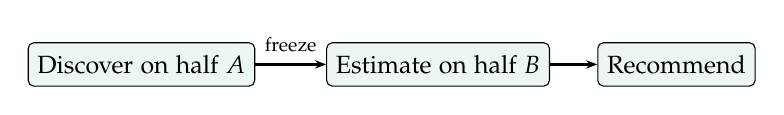
\begin{tikzpicture}[box/.style={draw,rounded corners=2pt,minimum height=0.55cm,font=\small,fill=greentint}]
\node[box](d){Discover on half $A$};
\node[box,right=0.9cm of d](e){Estimate on half $B$};
\node[box,right=0.6cm of e](r){Recommend};
\draw[a](d)--node[above=1pt,font=\scriptsize]{freeze}(e); \draw[a](e)--(r);
\end{tikzpicture}
\end{center}

\term{Causal forest} An average of honest trees. For a target $x$, the forest weights unit $i$ by
$\alpha_i(x) = \frac1B\sum_b \ind{X_i \in L_b(x)}/|L_b(x)|$ and solves a weighted residual regression:
\keybox{\hatt(x) = \frac{\sum_i \alpha_i(x)\,(Y_i - \hat\ell(X_i))(D_i - \hat e(X_i))}{\sum_i \alpha_i(x)\,(D_i - \hat e(X_i))^2}}

% ================================================================================================
\section{Evaluating CATE models and policies (Meeting 4, Block B)}

\term{Calibration test} Regress the held-out pseudo-outcome $\phi$ on the centered prediction,
$\phi = \beta_1 + \beta_2(\hatt(X) - \E[\hatt(X)]) + u$. Then $\beta_1 = \ATE$ and
$\beta_2 = \Cov(\tau(X), \hatt(X))/\Var(\hatt(X))$. A slope $\beta_2 = 1$ means calibrated, and $\beta_2 = 0$ means no
heterogeneity was found.

\term{GATES} Sort held-out units by $\hatt$ into $K$ groups with cut-points fixed in advance, and estimate each group's
average effect. Increasing group effects show the model ranks.
\remark{Variable importance is not a test: it says which variables the trees split on, not whether effects really vary.}


\term{Policy value} A policy is a rule $\pi: x \mapsto \{0,1\}$. Its gain over treating no one is
\keybox{G(\pi) = \E[\pi(X)\,v(X)] = \Pr(\pi(X) = 1)\cdot\E[v(X) \mid \pi(X) = 1]}
reach times the average net value of those it treats.

\term{IPW value} With a known propensity $e(x)$ and reward $R$,
\keybox{G(\pi) = \E\!\left[\pi(X)\left\{\frac{DR}{e(X)} - \frac{(1-D)R}{1-e(X)}\right\}\right]}
so any frozen policy can be scored on randomized data it was not chosen on.

\term{Freeze, then evaluate} The policy chosen as best on a selection sample looks better there than it is:
$\E[\hat G_S(\hat\pi)] \ge \E[G(\hat\pi)]$. On an independent evaluation sample its estimate is unbiased.

\term{Paired comparison} Compare two frozen policies on the same rows: with $d_i = g_i(\pi_a) - g_i(\pi_b)$, $\bar d$ is
unbiased for $G(\pi_a) - G(\pi_b)$ with $\SE = \text{sd}(d_i)/\sqrt n$, far smaller than two separate standard errors.

\term{Curves} The gain curve plots cumulative gain as more of the ranked list is treated; the profit curve subtracts costs and
peaks where the marginal unit's net value is zero. Gain curves and RATEs depend only on the ranking.

\term{RATE} With $\text{TOC}(q) = \E[\tau(X) \mid s(X) \text{ in the top } q] - \ATE$,
\keybox{\text{RATE} = \int_0^1 w(q)\,\text{TOC}(q)\,dq}
$w(q) = 1$ gives the AUTOC (the top of the list matters); $w(q) = q$ gives the Qini coefficient (the whole list). A random
ranking has $\text{RATE} = 0$.

\term{Ranking is not calibration} A threshold rule $\ind{s(x) > t}$ needs the score's level, not only its order. Isotonic
calibration fits a non-decreasing map $h$ of the score to (pseudo-)outcomes on a calibration sample; it never reverses the
order and is constant on blocks of scores.
\remark{Estimate rates within a group, then scale by its size. The raw difference in counts is biased, and even with equal arms
it is only half the group's incremental outcome.}

% ================================================================================================
\section{Allocation and decision (Meeting 5)}

\term{Unconstrained rule} Treat iff $v(X_i) > 0$; with a uniform cost, iff $\tau(X_i) > c/m$. If the cost is $k$ per unit sent
and $a$ per redemption, $v(x) = (m - a)\,\tau(x) - a\,\mu_0(x) - k$: sure things cost money.

\term{Caps and budgets} Under a cap of $B$ treatments, treat the $B$ largest positive $v_i$. Under a budget, rank by value
per yuan: greedy solves the relaxation and treats $i$ iff $b_i > (1+\lambda^\ast)c_i$.
\keybox{\frac{dV(C)}{dC} = \lambda^\ast \quad \text{(the shadow price of the budget)}}
\remark{Greedy is exact only for divisible units; with whole units it can miss the optimum (the 0--1 knapsack).}

\term{Group constraints} A cap on the treated-rate ratio between groups gives group-specific thresholds,
$\lambda^\ast + \eta^\ast/N_a$ and $\lambda^\ast - \gamma\eta^\ast/N_b$. The value lost to the constraint is its price.

\term{Spending risk} With independent redemptions at rates $s_i$, cost $K$ has $\E[K] = \sum_i d_ic_i$ and $\Var(K) = a^2\sum_i d_is_i(1-s_i)$;
keep $\Pr(K > C) \le \alpha$ by reserving $z_\alpha\sqrt{\Var(K)}$. A conservative rule treats a unit only if a lower confidence
bound on $v$ is positive; it treats a unit with $v \le 0$ with probability at most $\alpha$.

\term{Capacity} A nonlinear payoff needs each arm's outcome distribution, not only $\tau(x)$. To plan capacity $q$ with costs
$c_u$ per unit short and $c_o$ per unit over, choose the $\kappa$-quantile of $F_1(\cdot \mid x)$:
\keybox{\kappa = \frac{c_u}{c_u + c_o}}

% ================================================================================================
\section{Observational data (Meeting 6)}

\term{Three assumptions} Conditional exchangeability $\{Y(0), Y(1)\} \indep D \mid X$; overlap $0 < e(x) < 1$ on the target
population; consistency $Y = Y(D)$. Only overlap can be checked in the data.

\term{Standardization (g-formula)} $\E[Y(d)] = \E_X[\mu_d(X)]$, so $\ATE = \E_X[\mu_1(X) - \mu_0(X)]$ and
$\ATT = \E[Y - \mu_0(X) \mid D=1]$.

\term{Inverse probability weighting} $\E[DY/e(X)] = \E[Y(1)]$ and $\E[(1-D)Y/(1-e(X))] = \E[Y(0)]$. For the ATT, controls are
weighted by the odds $e(X)/(1-e(X))$. Normalize weights within each arm (H\'ajek). The effective sample size
$(\sum_i w_i)^2/\sum_i w_i^2$ shows how many units the comparison rests on.

\term{Balancing property} $D \indep X \mid e(X)$: one number, the propensity score, can replace all of $X$.

\term{What regression estimates} With effects that vary, the OLS coefficient on $D$ weights them by $e(X)(1-e(X))$:
$\E[\tau(X)\,e(X)(1-e(X))]/\E[e(X)(1-e(X))]$, which is neither the ATE nor the ATT.

\term{AIPW} The doubly robust score, averaged:
\keybox{\begin{aligned}\hatt_{\text{AIPW}} = \frac1n\sum_i \Big[&\tilde\mu_1(X_i) - \tilde\mu_0(X_i)\\ &+ \frac{D_i(Y_i - \tilde\mu_1(X_i))}{\tilde e(X_i)} - \frac{(1-D_i)(Y_i - \tilde\mu_0(X_i))}{1-\tilde e(X_i)}\Big]\end{aligned}}
consistent if either the outcome models or the propensity model is right; its score is the pseudo-outcome behind the
DR-learner of Meeting 3. It does not protect against an unmeasured confounder.

\term{Good and bad controls}

\begin{center}
\small
\begin{tabular}{@{}L{2.35cm}L{4.15cm}L{1.6cm}@{}}
\toprule
\textbf{Variable} & \textbf{Role} & \textbf{Adjust?} \\
\midrule
Confounder & causes $D$ and $Y$ & yes \\
Mediator & caused by $D$, causes $Y$ & no (total effect) \\
Collider & caused by $D$ (or a cause of $D$) and $Y$ & \textcolor{warnred}{no} \\
M-bias variable & pre-treatment, but a collider of two hidden causes & \textcolor{warnred}{no} \\
Cause of $D$ only & instrument-like; adjusting only adds variance & no \\
\bottomrule
\end{tabular}
\end{center}

\term{Overlap and trimming} Look at $\hat e(X)$ by arm and at the largest weights. Trimming to $\hat e \in [a, 1-a]$ stabilizes the
estimate but changes the estimand to the trimmed population; report it as such.

\term{Design before analysis} Without looking at outcomes: reconstruct the assignment mechanism; check overlap and fix the
trimming rule; fix the estimand this implies and the estimator; check balance after weighting; record the design with a date.
Only then open the outcomes.
\remark{Sensitivity: ask how strong an unmeasured confounder would have to be to move the estimate past the break-even.}

% ================================================================================================
\section{Double machine learning (Meeting 7)}

\term{Partially linear model} $Y = \theta D + g(X) + \varepsilon$ with $\E[\varepsilon \mid D, X] = 0$ and
$\E[\Var(D \mid X)] > 0$. With $\ell(x) = \E[Y \mid X=x]$ and $r(x) = \E[D \mid X=x]$ (Frisch--Waugh--Lovell),
\keybox{\theta = \frac{\E[(D - r(X))(Y - \ell(X))]}{\E[(D - r(X))^2]}}

\term{Why plug-in machine learning fails} Two biases appear, regularization bias (learners trade bias for variance) and
overfitting bias (nuisance models scoring the rows they were fitted on). The fixes:
\begin{itemize}
  \item \textbf{Orthogonality}: residualizing both $Y$ and $D$ makes the main error a product of the two models' errors, so
  moderate errors in each barely move $\hat\theta$. The treatment model's own error still attenuates $\hat\theta$: it must be good.
  \item \textbf{Cross-fitting}: every residual comes from models fitted on other folds.
\end{itemize}

\term{The DML algorithm} Split rows into $K$ folds at the level of any dependence (clusters, dates). For each fold, fit $\hat\ell$
and $\hat r$ on the other folds and form $\tilde Y_i = Y_i - \hat\ell(X_i)$, $\tilde D_i = D_i - \hat r(X_i)$. Then
\keybox{\hat\theta = \frac{\sum_i\tilde D_i\tilde Y_i}{\sum_i\tilde D_i^2}, \qquad \widehat\SE(\hat\theta) = \frac{\sqrt{\sum_i\tilde D_i^2\hat\varepsilon_i^2}}{\sum_i\tilde D_i^2}}
with $\hat\varepsilon_i = \tilde Y_i - \hat\theta\tilde D_i$; with clusters, sum $\tilde D_i\hat\varepsilon_i$ within each
cluster first.

\term{What $\theta$ averages} If the slope varies, $\hat\theta \to \E[\theta(X)\Var(D \mid X)]/\E[\Var(D \mid X)]$: units whose
treatment varies most count most. For a binary treatment and the ATE, use the interactive model and the AIPW score.

\term{Omitted-variable bound} If a hidden $U$ would explain shares $R^2_D$ of the residual treatment variance and $R^2_Y$ of
the residual outcome variance,
\keybox{|\text{bias}| \le \sqrt{\frac{R^2_Y\,R^2_D}{1 - R^2_D}}\cdot\frac{\text{sd}(\tilde Y - \theta\tilde D)}{\text{sd}(\tilde D)}}
\remark{Benchmark $R^2_D$ and $R^2_Y$ against a measured variable: ``a confounder as strong as this one would move the
estimate by at most\ldots''.}

% ================================================================================================
\section{Policy learning from observational data (Meeting 8)}

\term{Empirical welfare maximization} In logs, the doubly robust score $\phi_i$ uses an estimated propensity and outcome
models fitted on other folds (Meetings 6 and 7). Its net-value version $\Gamma_i = m\,\phi_i - c(X_i)$ has
$\E[\Gamma_i \mid X_i] = v(X_i)$, so choose the policy with the largest estimated gain in a class $\Pi$:
\keybox{\hat\pi = \arg\max_{\pi \in \Pi}\ \frac1n\sum_{i=1}^n \pi(X_i)\,\Gamma_i}
This is weighted classification, predicting the sign of $\Gamma_i$ with each unit weighted by $|\Gamma_i|$. A depth-two
policy tree is a readable class $\Pi$.

\begin{center}
\small
\begin{tabular}{@{}L{2.25cm}L{3.1cm}L{2.85cm}@{}}
\toprule
\textbf{Route} & \textbf{Learns} & \textbf{Trained to} \\
\midrule
Predict-then-optimize & $\hatt(x)$, then plugs in & predict well \\
Decision-focused & a model inside the optimizer & decide well with it \\
Policy learning & the rule $\pi$ directly & maximize estimated value \\
\bottomrule
\end{tabular}
\end{center}

\term{Regret} The oracle treats $x$ iff $v(x) > 0$. For any policy,
\keybox{V(\pi^\ast) - V(\pi) = \E\big[\,|v(X)|\;\ind{\pi(X) \ne \pi^\ast(X)}\big]}
only misclassified units cost anything, in proportion to their net value.
\remark{A richer class fits noise in the scores. Deploy a learned policy with a randomized holdout; a bandit makes it adaptive.}

% ================================================================================================
\section{Generative AI in causal analysis (Meeting 9)}

\subsection{Learned simulators}

\term{Simulator} A generative model fitted in causal order, $\hat p(x)$, $\hat p(d \mid x)$, $\hat p(y \mid d, x)$. Sampling $y$
for a chosen $d$ gives potential outcomes for any policy.

\term{Its effects are g-formula effects} If the pieces are exact, the simulator's average outcome under $d$ is
$\sum_x \E[Y \mid D=d, X=x]\,p(x)$: it equals $\E[Y(d)]$ exactly when the g-formula does. Realism is evidence about the data,
not about causation.

\term{Planted truth} To test methods, keep $\hat p(x)$ and a control-outcome model, and define treated outcomes as control
outcomes plus a chosen effect; a hidden confounder of chosen strength can be planted the same way. Two uses:
\begin{itemize}
  \item \textbf{estimator testbed}: bias and coverage of each method on data shaped like yours;
  \item \textbf{pipeline testbed}: run the whole predict-then-optimize pipeline and measure its regret against the oracle
  (Meeting 8).
\end{itemize}

\remark{Check a simulator with backtests against past experiments, stay within the data's support, watch errors compound
over many steps, and rank pipelines across simulators of different model classes (``home advantage''). A language model
asked for counterfactuals (silicon samples) asserts the truth from its priors; nobody planted it.}

\subsection{Language models as variable generators}

\term{A model-coded variable is a measurement} Its error matters through the variable's role:

\begin{center}
\small
\begin{tabular}{@{}L{1.9cm}L{6.2cm}@{}}
\toprule
\textbf{Role} & \textbf{What error does} \\
\midrule
Outcome & non-differential error (rates $\alpha, \beta$) scales the effect by $1-\alpha-\beta$; error that differs by arm can
create an effect from nothing \\
Modifier & symmetric misclassification $q$ shrinks heterogeneity by $1-2q$ \\
Control & embeddings work as DML controls, unless the text was written after treatment (leakage) or overlap collapses \\
\bottomrule
\end{tabular}
\end{center}

\term{Prediction-powered inference} With model labels $f_i$ on $N$ units and gold labels on $n$ of them,
\keybox{\hat\theta_{\text{PP}} = \frac1N\sum_{i=1}^N f_i + \frac1n\sum_{i \in \text{gold}}(Y_i - f_i)}
is unbiased for $\E[Y]$ whatever the model's quality; with an independent gold sample, its variance is
$\Var(f)/N + \Var(Y - f)/n$.
\remark{Check label accuracy separately in each arm: the gold sample must cover treated and untreated units.}

% ================================================================================================
\section{Panel data and difference-in-differences (Meeting 10)}

\term{Adoption-date outcomes} $Y_{it}(g)$ is unit $i$'s outcome in period $t$ if first treated in period $g$; $g = \infty$ means
never treated.

\term{Before--after fails} If units are treated because their outcome was unusually low, the change after treatment adds the
common trend and a regression to the mean: $\ATT + (\lambda_{\text{post}} - \lambda_{\text{pre}}) - \E[u_{\text{pre}} \mid T=1]$.

\term{Assumptions} Parallel trends: $\E[Y_{\text{post}}(0) - Y_{\text{pre}}(0) \mid T=1] = \E[Y_{\text{post}}(0) - Y_{\text{pre}}(0) \mid T=0]$.
No anticipation and no spillovers.

\term{DiD identifies the ATT}
\keybox{\begin{aligned}\ATT = {}&\{\E[Y_{\text{post}} \mid T=1] - \E[Y_{\text{pre}} \mid T=1]\}\\ &- \{\E[Y_{\text{post}} \mid T=0] - \E[Y_{\text{pre}} \mid T=0]\}\end{aligned}}
\remark{Parallel trends depends on the scale: if it holds in levels and the groups start at different levels, it fails in logs.}

\begin{center}
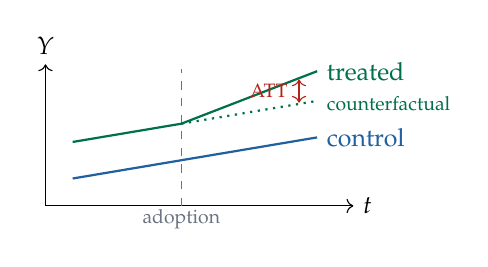
\begin{tikzpicture}[x=1.15cm,y=0.58cm,font=\small]
\draw[->](0,0)--(3.4,0) node[right]{$t$}; \draw[->](0,0)--(0,3.1) node[above]{$Y$};
\draw[dashed,extgrey](1.5,0)--(1.5,3); \node[extgrey,font=\scriptsize] at (1.5,-0.3){adoption};
\draw[thick,noteblue](0.3,0.6)--(1.5,1.0)--(3,1.5); \node[noteblue,right] at (3,1.5){control};
\draw[thick,sbgreen](0.3,1.4)--(1.5,1.8)--(3,2.95); \node[sbgreen,right] at (3,2.95){treated};
\draw[thick,sbgreen,dotted](1.5,1.8)--(3,2.3); \node[sbgreen,right,font=\scriptsize] at (3,2.25){counterfactual};
\draw[<->,warnred](2.8,2.26)--(2.8,2.77); \node[warnred,left,font=\scriptsize] at (2.78,2.52){ATT};
\end{tikzpicture}
\end{center}

\term{Regression form} Two-way fixed effects (TWFE) regress $Y_{it}$ on unit effects, period effects, and $D_{it}$. In a balanced
panel with one adoption date, its coefficient equals the DiD of unit averages. An event study replaces $D_{it}$ by indicators
for each period relative to adoption, except a base $k = -1$: post coefficients trace the effect, pre coefficients are placebos.

\term{Breakdown drift} If the counterfactual gap drifts by $\delta$ per period, the DiD estimates
$\ATT + \delta(\bar t_{\text{post}} - \bar t_{\text{pre}})$. The decision against break-even $c$ flips at
\keybox{\delta^\ast = \frac{\text{DiD} - c}{\bar t_{\text{post}} - \bar t_{\text{pre}}}}

\term{Inference} Cluster at the level of assignment. With independent units, collapse to one change per unit,
$\Delta_i = \bar Y_{i,\text{post}} - \bar Y_{i,\text{pre}}$, and compare groups: $\SE = \sqrt{s_1^2/n_1 + s_0^2/n_0}$.
\remark{With staggered adoption, TWFE also compares late adopters with early adopters whose effects are still changing; use
cohort-by-period effects $\ATT(g,t)$ against never- or not-yet-treated units instead.}

% ================================================================================================
\section{Synthetic control (Meeting 11)}

\term{Synthetic control} For one treated unit and $J$ donors, choose weights to fit the pre-period:
\keybox{\min_{w}\ \sum_{t=1}^{T_0}\Big(Y_{1t} - \sum_j w_jY_{jt}\Big)^2 \quad \text{s.t. } w_j \ge 0,\ \sum_j w_j = 1}
then $\hat Y_{1t}(\infty) = \sum_j w_jY_{jt}$ and $\hatt_t = Y_{1t} - \hat Y_{1t}(\infty)$ for $t > T_0$.

\term{Why it can work} If $Y_{jt}(\infty) = \delta_t + \lambda_t^\top\mu_j + \varepsilon_{jt}$ and the weights match the
treated unit's characteristics, $\sum_j w_j\mu_j = \mu_1$, the synthetic control is unbiased in every period, before and after.
The weights interpolate, so a treated unit outside the donors' range cannot be fitted.

\term{Design before the post-period} Freeze the donor pool, the fitting window, and the predictors before looking at
post-period outcomes; hold out the last pre-periods to check the fit.

\term{Placebos} Apply the method to every donor as if treated and rank the ratios $\text{RMSPE}^{\text{post}}/\text{RMSPE}^{\text{pre}}$.
The rank is an exact $p$-value, $k/(J+1)$, only if the treated unit was chosen at random; otherwise it is descriptive. Also use
in-time placebos (a fake adoption date) and leave-one-out (drop each donor in turn).

\begin{center}
\small
\begin{tabular}{@{}L{2.2cm}L{2.5cm}L{3.5cm}@{}}
\toprule
& \textbf{DiD} & \textbf{Synthetic control} \\
\midrule
Units weighted & equally & to fit the pre-period \\
Needs & parallel trends & a good pre-period fit \\
Best for & many treated units & one or a few treated units \\
\bottomrule
\end{tabular}
\end{center}
\remark{Synthetic DiD combines unit weights with time weights; matrix completion imputes the missing untreated outcomes from
a low-rank panel.}

% ================================================================================================
\section{Further designs (not examined)}

\term{Instruments not randomized} An outside shifter $Z$ of treatment must be independent of potential outcomes (argued, not
designed), relevant, excluded, and monotone. Two-stage least squares then estimates a LATE, weighted across strata. Weak
instruments bias it toward the naive regression; $F > 10$ is a floor, not a certificate, and the Anderson--Rubin test keeps its
size at any strength.

\term{Regression discontinuity} If treatment switches at a cut-off $c$ of a running variable $R$, and potential outcomes are
continuous at $c$, the jump $\lim_{r \downarrow c}\E[Y \mid r] - \lim_{r \uparrow c}\E[Y \mid r]$ is the effect at $c$. A fuzzy
design divides by the jump in treatment. Check the density of $R$ and covariates at the cut-off.

\term{Interference} When units affect each other, a unit-randomized test estimates a direct effect at the current saturation,
not the global effect of treating everyone; cluster or switchback designs target the global effect.

\term{Sequential decisions} When a response to the first action informs the second, value a regime with the sequential
g-formula, learn it by Q-learning, and evaluate logged policies by IPW or doubly robust estimators. Never adjust for the
intermediate response.

\end{multicols*}
\end{document}
